\chapter*{Programme officiel}

\section*{Programme officiel}

Les données organisées en table correspondent à une liste de p-uplets nommés qui partagent les mêmes descripteurs. La mobilisation de ce type de structure de données permet de préparer les élèves à aborder la notion de base de données qui ne sera présentée qu'en classe terminale. Il s'agit d'utiliser un tableau doublement indexé ou un tableau de p-uplets, dans un langage de programmation ordinaire et non dans un système de gestion de bases de données.

{\centering\begin{tabular}{|L{3cm}|L{5.5cm}|L{6cm}|}\hline
\cellcolor{bo}\bfseries\textcolor{white}{Contenus}&
\cellcolor{bo}\bfseries\textcolor{white}{Capacités attendues}&
\cellcolor{bo}\bfseries\textcolor{white}{Commentaires}\\ \hline
Indexation de tables
&
Importer une table depuis un fichier texte tabulé ou un fichier CSV.
& Est utilisé un tableau doublement indexé ou un tableau de p-uplets qui partagent les mêmes descripteurs.\\ \hline
Recherche dans une table
&
Rechercher les lignes d'une table vérifiant des critères exprimés en logique propositionnelle.
&
La recherche de doublons, les tests de cohérence d'une table sont présentés.\\ \hline
Tri d'une table
&
Trier une table suivant une colonne.
&
Une fonction de tri intégrée au système ou à une bibliothèque peut être utilisée.\\ \hline
Fusion de tables
&
Construire une nouvelle table en combinant les données de deux tables.
&
La notion de domaine de valeurs est mise en évidence.\\ \hline
\end{tabular}\par}


\chapter{Indexation de tables}

\section{Open data}

\Cours{{\bfseries Open data}

Un contenu est dit en \emph{open data} s'il est librement utilisable, modifiable et partageable par n'importe qui et pour n'importe quelle raison.}

\begin{itemize}
	\item En France, \href{https://www.etalab.gouv.fr/}{Etalab} s'occupe de \href{https://www.data.gouv.fr/fr/}{data.gouv.fr}, site de partage des données publiques.
	
	%\item Citoyenneté. Par exemple : ce que les laboratoires pharmaceutiques donnent à nos médecins, \href{http://www.regardscitoyens.org/sunshine/}{regardscitoyens.org/sunshine/}.
	\item Des données sont également disponibles localement, par exemple : \href{data.larochesuryon.fr}{data.larochesuryon.fr}.
    \item Certaines données sont collaboratives, par exemple : \href{https://fr.openfoodfacts.org/}{fr.openfoodfacts.org} autour des produits alimentaires ou \href{https://www.openstreetmap.fr/}{openstreetmap.fr} sur la cartographie.
\end{itemize}

Les formats de données les plus courants sont CSV et JSON.

Prenons l'exemple de \href{https://www.data.gouv.fr/fr/datasets/fete-de-la-musique-2019/}{https://www.data.gouv.fr/fr/datasets/fete-de-la-musique-2019/}

Ce sont deux fichiers lisibles par n'importe quel éditeur de texte... 
	
	{\centering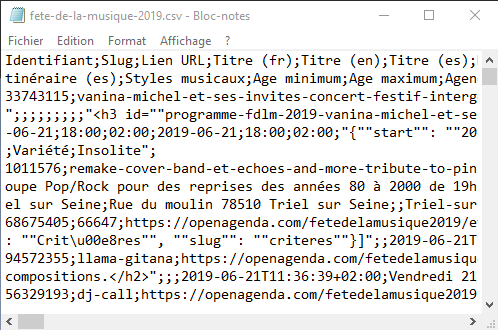
\includegraphics[height=4cm]{images/fetecsv.png} \qquad 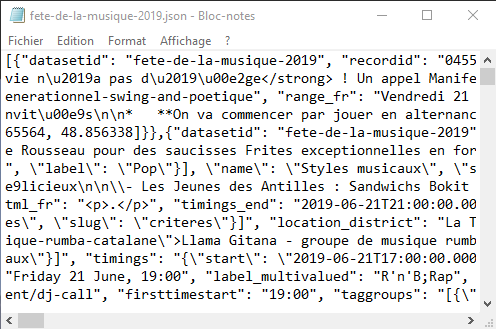
\includegraphics[height=4cm]{images/fetejson.png}\par}
	
	mais difficilement pour un humain, il y a un peu de travail !

Il existe cependant des outils pour nous aider (tableur : CSV, et navigateur web : JSON) :
	
	{\centering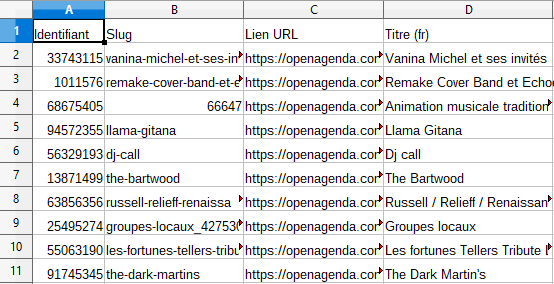
\includegraphics[height=3.5cm]{images/fetecsv2.png} \qquad 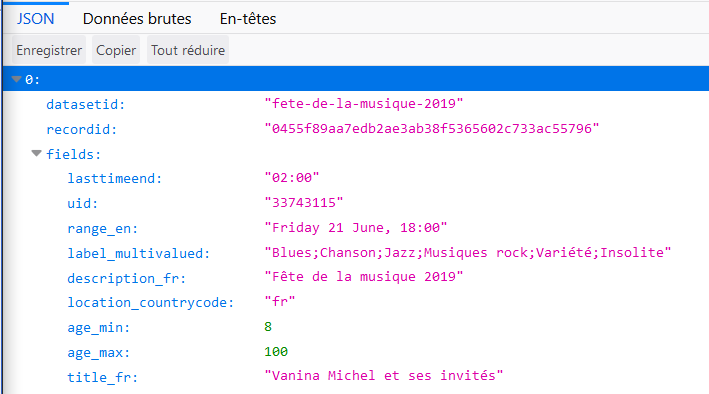
\includegraphics[height=3.5cm]{images/fetejson2.png}\par}

Si on regarde la première ligne du JSON : 

\texttt{[\{"datasetid": "fete-de-la-musique-2019", "recordid": "0455f89aa7edb2ae3}$\cdots$

on peut reconnaitre les formatage de listes et de dictionnaires Python. C'est ça qui permet de comprendre ce format. Si on regarde les deux premières lignes du CSV :

\texttt{Identifiant;Slug;Lien URL;Titre (fr);Titre (en);Titre (es);}$\cdots$

\texttt{33743115;vanina-michel-et-ses-invi}$\cdots$\texttt{ique;https://open}$\cdots$

La structure est beaucoup plus pauvre : 

\begin{itemize}
 \item Il n'y a qu'un séparateur (ici le << \texttt{;} >>).  
 \item La première ligne est réservée aux \emph{descripteurs}.
 \item Chacune des lignes suivantes correspond à une donnée définie par les valeurs correspondantes à ces descripteurs.
\end{itemize}

\medskip

Le but de cette partie est de traiter les données en tables donc au format CSV. Pour le format JSON, comme dit plus haut, on utilise un dictionnaire.

\section{Lecture/écriture d'un fichier texte}

Une table CSV est avant tout un fichier texte avec un certain format. 

Le langage Python dispose d'une fonction \pythoninline{open()} pour ouvrir un fichier en mode texte. 

Il dispose également d'une méthode \pythoninline{close()} pour le fermer :

\begin{multicols}{2}
\begin{minted}{python}
fichier = open('fichier.txt', 'w')
for i in range(1,4):
    fichier.write('Ligne '+srt(i)+'\n')
fichier.close()
\end{minted}

L'argument \pythoninline{'w'} pour << write >> ouvre (quitte à le créer) le fichier en écriture. Cet argument est \pythoninline{'r'} pour << read >> (ouverture en lecture) par défaut, et peut aussi être \pythoninline{'a'} pour << append >> (ouverture en ajout).
\end{multicols}

Pour éviter les problèmes de non-fermeture de fichier ouvert (si par exemple l'exécution du programme s'interrompt avant) on utilise le mot clé \pythoninline{with} qui gère le problème :

\begin{minted}{python}
with open('fichier.txt') as fichier :
    print(fichier.read())
\end{minted}

\begin{itemize}
	\item \pythoninline{fichier.read()} revoit une chaine de caractère contenant le fichier entier.
	\item \pythoninline{fichier.readlines()} aurait séparé chaque ligne dans une liste.
	
	\item On peut aussi itérer sur le fichier pour ne charger qu'une ligne en mémoire à la fois :

\begin{minted}{python}
with open('grosfichier.txt') as fichier :
    for ligne in fichier :
        print(ligne)
\end{minted}
\end{itemize}


Supposons disposer du fichier \texttt{notes.txt} contenant les trois lignes ci-dessous.

\begin{multicols}{2}

\vspace{-2ex}
\begin{minted}{text}
Nom;DS1;DS2;DS3;DS4;DS5
Bob;10;12;5;14;13 
Rick;12;10;ABS;12;11
\end{minted}

Si on perçoit les données comme un tableau à deux dimensions, on peut les extraire comme présenté ci-contre.

\pythoninline{ligne.rstrip('\r\n')} permet de nettoyer les fins de lignes et \pythoninline{ligne.split(';')} permet de créer une liste en séparant la chaîne au niveau des \pythoninline{';'}.

\begin{minted}{python}
# Extraction
notes = []
with open('notes.txt') as fnotes :
    for ligne in fnotes :
        ligne = ligne.rstrip('\r\n')
        notes.append(ligne.split(';'))

# Génération de l'index
index = {}
for (i, idx) in enumerate(notes[0]) :
    index[idx] = i
del(notes[0])
\end{minted}

\end{multicols}

La première ligne contenait les index. On répertorie leurs indices dans le dictionnaire \pythoninline{index} ( \pythoninline|= {'Nom' : 0, 'DS1' : 1,|...) et on la supprime du tableau de données \pythoninline{del(notes[0])}.

A présent la note de Bob au DS3 est \pythoninline{notes[0][index['DS3']]}.

\section{Importer une table CSV}

Les séparateurs \pythoninline{';'} et \pythoninline{'\r\n'} ne sont pas les seuls possibles. De plus, une des données à séparer pourrait être un texte comportant ces symboles... Une << bonne >> écriture d'extraction d'un fichier CSV est donc bien plus délicate à produire. Heureusement elle existe déjà dans la bibliothèque du même nom.

\medskip

Avec notre fichier \texttt{notes.txt}, cela donne :

\begin{minted}{python}
# Extraction
import csv

notes = []
with open('notes.csv') as fnotes:
    csvnotes = csv.reader(fnotes, delimiter=';')
    for ligne in csvnotes:
        notes.append(ligne)
\end{minted}

Les traitements comme  \pythoninline{ligne.replace('\n','')} ou
\pythoninline{ligne.split(';')} sont tous contenues dans \pythoninline{csv.reader()} et le rendu correspond aux listes attendues. 

\medskip


On peut avoir besoin de préciser l'encodage du texte en argument de la fonction \pythoninline{open()}. Pour le fichier \texttt{fete-de-la-musique-2019.csv} donné en exemple au début on pourra écrire :
\pythoninline{open('fete-de-la-musique-2019.csv', encoding='utf8')}

\medskip

{\bfseries Pour aller plus loin :}
Avec un fichier JSON, on peut utiliser la bibliothèque du même nom, et on obtient une liste de dictionnaires avec :

\vspace{-2ex}
\begin{minted}{python3}
import json

with open('fete-de-la-musique-2019.json', encoding='utf8') as ffete:
    fete = json.loads(ffete.read())
\end{minted}

\chapter{Manipulation de tables}

Il existe des modules pour le traitement de données issues de tables, comme \pythoninline{pandas}. Le parti pris pour la suite est de ne pas les utiliser. On considèrera donc les << tables >> de données comme étant des listes de listes ou de p-uplets Python  (on peut inclure les dictionnaires, si l'ordre n'a pas d'importance). 

L'exemple utilisé vient du fichier \texttt{fete-de-la-musique-2019.csv}, téléchargeable sur :

\href{https://www.data.gouv.fr/fr/datasets/r/49234ba7-00cd-401a-bb7c-70b81806b3eb}{https://www.data.gouv.fr/fr/datasets/fete-de-la-musique-2019/}

Et on suppose avoir fait l'indexation suivante :

\vspace{-2ex}
\begin{minted}{python}
import csv

table = []
with open('fete-de-la-musique-2019.csv', encoding='utf8') as ffete:
    csvfete = csv.reader(ffete, delimiter=';')
    for ligne in csvfete:
        table.append(ligne)

index = {}
for (i, idx) in enumerate(table[0]) :
    index[idx] = i
del(table[0])
\end{minted}

\section{Recherche dans une table}



En open data, on a souvent de gros fichiers, apportant beaucoup plus d'informations que ce que l'on cherche réellement. Il est donc important de pouvoir les sélectionner. Sur l'exemple de la fête de la musique, on peut vouloir ne s'intéresser qu'à une ville. On parcourt toutes les lignes de données et on récupère celles qui satisfont à ce critère : 

\begin{minted}{python}
laRocheSurYon = []
for ligne in table :
    if ligne[index['Ville']] == 'La Roche-sur-Yon' :
        laRocheSurYon.append(ligne)
\end{minted}

Il suffit de pouvoir exprimer ce critère avec des expression booléennes (en logique propositionnelle) : on emploie à loisir les \pythoninline{and},  \pythoninline{or},  \pythoninline{not}...

\medskip

On peut également vouloir filtrer certains index et donc supprimer certaines colonnes. Pour ce faire, on peut par exemple reconstruire une liste en sélectionnant ceux que l'on veut garder :

\begin{minted}{python}
simple = []
for ligne in laRocheSurYon :
    simple.append([ ligne[index['Titre (fr)']],
                    ligne[index['Nom du lieu']],
                    ligne[index['Première ouverture']] ])
\end{minted}

Une fois ces sélections effectuées (ou d'autres opérations), il peut arriver que certaines lignes soient identiques (par exemple, s'il ne reste plus que les valeurs de \texttt{Première ouverture} dans chaque ligne). On peut alors avoir besoin d'identifier/supprimer ces doublons.

On peut pour cela parcourir les données en recopiant celles qui ne l'ont pas déjà été :

\begin{minted}{python3}
unique = []
for ligne in simple:
    if ligne not in unique:
        unique.append(ligne)
\end{minted}

On peut améliorer ce code si la table était triée (les valeurs identiques seraient alors côte à côte.)

%%%%%%%%%%%%%%%%
%%%%%%|  |%%%%%%
%%%%%%|  |%%%%%%
%%%%%%|  |%%%%%%
%%%%\      /%%%%
%%%%%\    /%%%%%
%%%%%%\  /%%%%%%
%%%%%%%\/%%%%%%%
%%%%%%%%%%%%%%%%

{\color{rouge}\bfseries Tests de cohérence ?}

\section{Tri d'une table}

Des algorithmes de tri sont expliqués dans la partie algorithmique et peuvent bien sûr être appliqués. Pour ne pas surcharger, on propose ici d'utiliser la méthode \pythoninline{sort()} qui s'applique à une liste pour la trier selon une clé. Cette clé est une fonction qui prend en paramètre l'élément à trier et renvoie la valeur de cet élément dans ce tri :

\begin{minted}{python}
# On va trier selon la colonne d'indice 2
def valeurPourTrier(ligne):
    return ligne[2]

simple.sort(key = valeurPourTrier)
\end{minted}

On peut trier selon plusieurs critères, en faisant renvoyer un p-uplet comme clé.

On obtient un ordre total selon toutes les colonnes dans l'ordre si on ne précise pas de clé.
(L'amélioration de la suppression de doublon est alors possible...)

%
%Si hachable
%
%liste = [7, 8, 9, 5, 1, 7, 9, 5, 6, 2, 5, 3, 1, 4, 3, 2, 1]
%dictemp = {}
%newlist = [dictemp.setdefault(e,e) for e in liste if e not in dictemp]

\section{Fusion de tables}

On suppose disposer de deux tables comportant un champ en commun. Leur fusion consiste à les réunir en une seule table regroupant toutes les informations.

Prenons un exemple simple de deux tables déjà chargées et filtrées :

\begin{multicols}{2}

\begin{minted}[firstnumber=1]{python3}
index1 = ['Prénom', 'age']
table1 = [['Pierre', 12],
          ['Paulette', 14],
          ['Jack', 13]]
\end{minted}

\begin{minted}[firstnumber=5]{python3}
index2 = ['nom', 'Prénom']
table2 = [['Dupond','Pierre'],
          ['Pagnol','Pauline'],
          ['Potter','Jack']]
\end{minted}
\end{multicols}

Le champ commun est \pythoninline{'Prénom'}.

Un premier algorithme pour répondre à cette demande : 

On prépare la fusion en créant les champs nécessaires à partir d'une de table,

\begin{minted}[firstnumber=10]{python3}
index = [*index2, index1[1]]
fusion = []
for i in range(len(table2)):
    fusion.append([*table2[i],-1])
\end{minted}

 puis on parcourt l'autre table en cherchant pour chaque enregistrement s'il y en a un qui correspond pour les fusionner.
 
\begin{minted}[firstnumber=14]{python3}
for i in range(len(table1)):
    fusionOK = False
    for j in range(len(fusion)):
        if fusion[j][1] == table1[i][0]:
            fusion[j][2] = table1[i][1]
            fusionOK = True
    if not fusionOK :
        fusion.append(['',*table1[i]])
\end{minted}

\begin{itemize}
	\item S'il y avait eu deux prénoms identiques, la construction serait faussée.
	
	Il est important que le champ commun identifie clairement chaque enregistrement.
	
	Il est sinon possible de prendre plusieurs champs commun pour assurer cette unicité.
	\item On voit que la première partie complète le champ vide avec \pythoninline{-1} alors que dans la seconde, il est complété avec \pythoninline{''}. Il est important pour des traitements  ultérieurs de conserver le type de donnée associé à un champ. En proposant \pythoninline{-1} pour un âge qui devrait être positif et \pythoninline{''} pour un Nom qui devrait être au moins un caractère, on se place juste en dehors du domaine de valeurs du champ, pour spécifier qu'il n'est pas connu.
\end{itemize} 

\medskip

Si les deux tables étaient triées selon la valeur du champ commun, un algorithme de fusion beaucoup plus efficace existe : il parcourt les deux tables en même temps et ajoute à la fusion, à chaque étape, l'enregistrement le plus petit s'ils diffèrent entre les deux tables, ou leur fusion s'ils sont identiques.